 \documentclass{MScthesisITEM}

% this package is just to generate text for demo-purposes

\usepackage{color}
\usepackage{parskip}
\usepackage{blindtext}
\usepackage{mathtools} % math packages
\usepackage{todonotes}
\usepackage{hyperref}
\usepackage{subcaption}
\usepackage{wrapfig}
\usepackage{pgfplots}
\usepackage{filecontents}
\usepackage{url}
\usepackage{float}
\usepackage{listings}
\usepackage{amsfonts}
\usepackage{amssymb}
\usepackage{csquotes}

\usepackage{float}
\usepackage{tikz}
\usetikzlibrary{positioning, fit, calc, shapes, arrows}
\usepackage{pgf-umlsd}
%\usepackage[procnames]{listings}

%\pgfplotsset{compat=1.11}
\setlength{\parindent}{0pt}

\definecolor{keywords}{RGB}{255,0,90}
\definecolor{comments}{RGB}{0,0,113}
\definecolor{red}{RGB}{160,0,0}
\definecolor{green}{RGB}{0,150,0}

\lstset{
	numbers=left,
	stepnumber=1, 
	numbersep=5pt,
	showspaces=false,
	showstringspaces=false,
	showtabs=false,
	basicstyle=\footnotesize, 
	numberstyle=\footnotesize, 
	tabsize=2, 
	breaklines=true,
	captionpos=b,}



\title{Identity-Based Trust Model in Named Data Networking} % The title of your assignement; NB use \newlinetitle to start a newline
\author{Haakon Garseg Mørk} % Your firstname and lastname
\professor{Stig F. Mjølsnes, ITEM} % Affiliation = ITEM for instance
\supervisor{N/A}

%% Uncomment the following in case you want subfigures; note that there will be a warning for the caption package
% \let\subcaption\undefined
% \let\subfloat\undefined
% \usepackage[bf]{caption}
% \usepackage{subcaption}

\DeclareGraphicsExtensions{.pdf,.jpg}
\graphicspath{{./figs/}}

\loadglsentries{glossary}
\makeglossaries

\begin{document}
\selectlanguage{english}
\pagenumbering{roman}
\pagestyle{plain}

%% Only for the project; comment out the line below for the master's thesis; the front page will be generated automatically by DAIM
%\titleITEM

%% Only for the master's thesis; for the project report the description is taken from It's Learning and added by the department
% \selectlanguage{english} % Change to 'norsk' if you are writing in Norwegian
% \begin{titlingpage}

\noindent
\begin{tabular}{@{}p{4cm}l}
\textbf{Title:} 	& Security Properties in Information-centric Networking \\
\textbf{Student:}	& Haakon Garseg Mørk \\
\end{tabular}

\vspace{4ex}
\noindent\textbf{Problem description:}
\vspace{2ex}

The translation from name to address and location is a fundamental problem to all networks.
Named Data Networking (NDN) is a proposal for content-centric discovery and routing approach to networking
going on at the University of California, Los Angeles (UCLA) [1], which is part of the inspiration and a contact point for this work.

This project aims to understand the ideas and concepts of named data networking, and investigate the
potential these notions hold for network security, even for properties of anonymity and privacy. 
The student work should be to build a public key distribution application that uses ChronoSync [2] and runs over NDN.
This approach will allow for easy experimentation in the regular internet protocols environment.     

[1]  UCLA.  Named Data Networking. Web site at http://named-data.net/

[2]  UCLA, Named-data Networking. ChronoSync https://github.com/named-data/ChronoSync

\noindent
\begin{tabular}{@{}p{4cm}l}
\textbf{Responsible professor:} 	& Stig F. Mjølsnes \\
\textbf{Supervisor:}			& Stig F. Mjølsnes \\
\end{tabular}

\end{titlingpage}
% \cleardoublepage

%% There must be an abstract in English, even though the main text is in Norwegian
\selectlanguage{english}
\pagestyle{empty}
\begin{abstract}
Intro ..

In this paper .. goals

Results .. 

Conclusion ..
\end{abstract}
\cleardoublepage

%% Only for the master's thesis; if the main text is in English and you can write Norwegian, there must be an abstract in Norwegian as well.
% \selectlanguage{norsk}
% \pagestyle{empty}
\begin{abstract}

IP nettverket ble bygd for flere ti\r{a}r siden, og med dagens bruk av Internet ser vi at en ny nettverksprotokoll er s\r{a}rt trengt.
Named Data Networking (NDN) er en foresl\r{a}tt nettverksprotokoll som baserer seg p\r{a} innhold, istedenfor punkt-til-punkt arkitekturen som er grunnlaget for IP.
Selv med flere ti\r{a}rs bruk av Internet, er enn\r{a} ikke problemene med Public Key Infrastructure (PKI) l\o{}st. 
I NDN, har man heller ikke klart \r{a} finne en l\o{}sning p\r{a} dette.
Identitetsbasert kryptografi (IBC) viser seg \r{a} være anvendelig til tr\r{a}dl\o{}se sensornettverk, og enda mer n\r{a}r sensornettverket kj\o{}rer over NDN.

I denne masteroppgaven forklarer jeg NDN arkitekturen og de grunnlegende prinsippene i IBC.
Jeg modellerer og implementerer en applikasjon for \r{a} demonstrere bruken av IBC over NDN i et tenkt sensornettverk.

Implementasjonen og testingen av mitt bidrag verifiserer relevansen av IBC i et sensornettverk som kj\o{}rer over NDN, samt brukervennligheten rundt det \r{a} utvikle applikasjoner over NDN.

Jeg formelt og uformelt beviser sikkerheten i protokollene som er foresl\r{a}tt til enhetsregistrering og data foresp\o{}rsel i applikasjonen.

\end{abstract}
% \cleardoublepage

\selectlanguage{english}% Change to 'norsk' if you are writing in Norwegian

% \include{preface}
% \cleardoublepage

\renewcommand{\abstractname}{Acknowledgments}
\begin{abstract}
Acknowledgment goes here
\end{abstract}
\cleardoublepage

% similarly you may add a separate acknowledgments page

\tableofcontents*
\cleardoublepage

%% include if relevant
\listoffigures
\cleardoublepage

\lstlistoflistings
\cleardoublepage

%% include if relevant
\listoftables
\cleardoublepage

%% include if relevant
%\listofalgorithms
%\addcontentsline{toc}{chapter}{List of Algorithms}
%\cleardoublepage

%% include if relevant
\printglossary[title=List of Terms, style=long]
\cleardoublepage
% \glsaddall[]

% include if relevant
\printglossary[title=List of Acronyms,type=\acronymtype] % prints just the list of acronyms
\cleardoublepage

\pagenumbering{arabic}
\pagestyle{ruled}
\chapter{Introduction}\label{chp:introduction} 

\section{Motivation}
The translation from name to address and location is a fundamental problem to all networks.
\gls{NDN} is a proposal for content-centric discovery and routing approach to networking
going on at the \gls{UCLA}, which is part of the inspiration and a contact point for this work.

In general, the name to address resolution can either be maintained by a catalogue lookup service, 
such as \gls{DNS} (Internet) and \gls{HLR} (mobile networks), 
or resolved on-the-fly by a protocol on request, such as \gls{ARP} (\gls{LAN}). 
There has been done a tremendous amount of work on the naming problem in distributed systems, 
some became big failures (e.g. X.500) others such as the web \gls{URL}s are very successful. 
Bringing things even further, the \gls{DOI} system is a \gls{URI} directed at the content/object itself rather than a location. 
Very much related to the name/address problem is the information security problem of efficient and practical public key distribution, 
which remain unsolved in practice, even though a significant number of digital certificate and verification protocols and schemes have been proposed, and systems tested over the last two decades. 
One notable and early theoretical proposal is Adi Shamir's \gls{IBC} proposal~\cite{DBLP:conf/crypto/Shamir84},
and subsequent work, that may be revisited and applicable to \gls{NDN}.

\section{Problem and Scope}

Designing a new network protocol for the future Internet, one of the most significant changes should be security.
Trust management plays a big part in security, and thus we cannot design trust management on known \gls{IP} failures such as X.500. 
\gls{PKI} is a tough challenge to solve and it is probably not a rigid solution, but rather case specific.
\gls{NDN} is being designed with security in mind, but the issue of trust management is yet to be solved.

In addition to the problem description, I also address the trust management issue in a thought sensor device network using \gls{IBC}.
By using the \gls{NFD} I will implement my proposal for such sensor network over \gls{NDN}, and contribute with ideas and concepts around such network.

\section{Methodology}

When developing applications over \gls{NDN} it is important to understand the architecture of the protocol. 
I will study the protocol, reading the guide for NDN developers~\cite{NDN-0021} and papers published by the \gls{NDN}-team\footnote{NDN Publications - http://named-data.net/publications/} describing protocol features in addition to existing applications running over \gls{NDN}.

The concept of \gls{IBC} should be thoroughly understood, as I will apply it in my application.
Thus I will study \gls{IBC}, finding relevant papers at Google Scholar\footnote{Google Scholar - https://scholar.google.no/}.

Establishing a solid background knowledge in these topics, I first design the application flow in sequence diagrams.
Based on the \gls{api} to the \gls{PyNDN2}, I try to implement the proposed design and see where changes can be made to minimize communication overhead, maximize security (i.e. \gls{CIA}) and maximize usability.
The implementation will be tested and cryptographic parameters will be measured.
I will prove the security in the protocols I propose and finally I will discuss the work done.

\section{Outline}

This thesis will first introduce \gls{NDN}, one of the proposed protocols for the future Internet.
I will explain the architecture of \gls{NDN} as well as some related work regarding my application proposal and \gls{IBC}. 
The concept of \gls{IBC} will also be explained.
The specifications for the \gls{HSS} application will be explained in detail and implementation choices will be discussed.
I will present the results of the implementation and testing.
At last, a discussion around the research topics in the thesis will be presented and finally my conclusion around the same topics.

\chapter{Background}\label{chp:background} 
\chapterprecishere{"We model the future on the past. Sometimes that’s a mistake."\par\raggedleft--- \textup{Van Jacobsen}, SIGCOMM 2001}

This chapter will give a brief overlook of the motivation for \gls{ICN}, as well as explaining more details of the \gls{ICN} protocol \gls{NDN}.
The \gls{NDN} architecture will be reviewed.
Finally there will be a quick summary of related work.

\section{Motivation for Information-Centric Networking}
When Internet was created in the 1960's, the researchers where inspired by the existing communication network; the telecommunication network.
Because it was natural and logical to think that people would send and receive short messages and instructions, the point-to-point communication model was a logical architecture. 
As Internet have developed, the traffic has increased enormously over the past few years. 
In the Global Internet Phenomena Report 1H2014 done by Sandvine~\cite{gipr2014}, close to 64\% of all \gls{IP} traffic in North America was Real-Time Entertainment streaming.
In~\autoref{fig:ip-traffic} it can easily be seen that most of the traffic is content download, and not communication as Internet was designed for.
With this in mind, the \gls{IP} architecture does not provide an efficient transport model for what we are actually using the network for.

\begin{figure}[ht]
  \centering
  \begin{subfigure}{0.5\textwidth}
    \centering
    \includegraphics[width=0.98\linewidth]{north-america-ip-traffic.png}
    \caption{North America}
    \label{fig:north-america-ip-traffic}
  \end{subfigure}%
  \begin{subfigure}{0.5\textwidth}
    \centering
    \includegraphics[width=0.98\linewidth]{europe-ip-traffic.png}
    \caption{Europe}
    \label{fig:europe-ip-traffic}
  \end{subfigure}
  \caption{
  (a) Peak Period Aggregate Traffic Composition - North America, Fixed Access~\cite{gipr2014}.
  (b) Peak Period Aggregate Traffic Composition - Europe, Fixed Access.
  }
  \label{fig:ip-traffic}
\end{figure}

Designing the \gls{IP} network, security was not the first priority.
A logical thought considering that they did not know what the Internet is being used for and how big it has become.
Many protocols related to Internet have been designed and deployed mainly with the goal of functionality, not thinking about security.
In the years after the birth of Internet, it was discovered that Internet needed security at several layers, due to that the application requirements and transmission importance increased.
\gls{IPsec} is a very good example of work trying to patch up security flaws in the design of Internet.

Today, WiFi is disseminated across homes and buildings in many countries. 
Wireless technology has grown rapidly and it is predicted continuous growth in the years to come.\todo{find a cite} 
The \gls{IoT} trend is coming and the \gls{IP} network is not designed for broadcast.
Therefore wireless connection is not as easy as it should and could be.
Devices should easily be able to communicate directly with each other without having to interconnect through a router.

Another problem is the network redundancy. 
Looking at~\autoref{fig:ip-traffic} and reading~\cite{gipr2014} where it comes to light that Netflix stands for 34.21\% of all content download in America, one can conclude that there are a lot of movies downloaded from \textit{x} users geographically located close.
And thus the network path from the source (e.g. Netflix) to this geographical place is allocated \textit{x} too many times. 
This is because a node in an \gls{IP} network does not know \textit{what} it processes, but rather the packet's endpoints, i.e. \textit{where} it goes and \textit{where} it comes from. 
This makes every node dumb, hence the network is designed for redundancy when it comes to content download.

These design failures are some the reasons why the research for the future Internet began.  
\gls{ICN}~\cite{DBLP:journals/cm/AhlgrenDIKO12} is a concept developed under this research.
It is built upon delivery of content, rather than the point-to-point model we previously have seen in \gls{IP}.
\gls{ICN}s goal is to build an infrastructure of a new Internet that can achieve efficient, secure and reliable distribution of content.
In 2012 \gls{IRTF} established \gls{ICN} working group.


\section{Content Centric Network \& Named Data Network}\label{chp2:sec:icn}
The first network protocol purposed for \gls{ICN}, \gls{CCN}, was presented by Van Jacobsen at a Google Talk in 2006. 
He, amongst other contributors of \gls{CCN}, has been working on developing the Internet as we know it since the early start.
Jacobsen has contributed to \gls{TCP}/\gls{IP} with his flow control algorithms~\cite{DBLP:conf/sigcomm/Jacobson88} and \gls{TCP} header compression~\cite{rfc1144}.
\gls{CCN} focuses on naming content, instead of naming \gls{IP}-addresses. 
The research project is lead by \gls{PARC}.
A branch of \gls{CCN} is the \gls{NDN}~\cite{DBLP:journals/ccr/0001ABJcCPWZ14} research project started in 2010, which Jacobsen also have contributed to.
One of the biggest contributers is \gls{UCLA}, with Lixia Zhang \todo{history on Zhang} in the lead. 
Zhang is known for her contribution to, amongst many other, \gls{RSVP}~\cite{rfc2205} and \gls{MACAW}~\cite{DBLP:conf/sigcomm/BharghavanDSZ94}.
The \gls{NDN} project is also one of few projects funded by \gls{NSF} in their \gls{FIA} program~\cite{nsf-fia}.

\section{NDN Architecture}\label{chp2:sec:ndn_architecture}
Since the knowledge of how \gls{NDN} works is not disseminated amongst computer scientists, it is essential for this thesis to describe how it works.
This section will describe the basic architecture of \gls{NDN}~\cite{NDN-0021} and compare some solutions with the equivalent solutions in \gls{IP}.

\subsection{Brief Introduction}
In \gls{NDN} there are two types of packets, Interest and Data packet.
All data has be given a content Name by its publisher. 
To publish some content to the network, a user have to register the prefix, i.e. announcing the contents Name, which tells the network that the content can be retrieved on the announced Name. 
The retrieval can only be achieved if someone expresses an Interest to the content Name.
If a user expresses Interest in the Name, the network will route the Interest to the closest node that holds the Data. 
The Data packet can be retrieved from any node, trusted or not, over any type of communication channel, secure or not. 
Finally the requester will receive the Data packet containing the content.
The Data can be verified by the requester ensuring that the publisher who ``owns'' the content actually is the owner, because its cryptographically signed.
It is because of the signature we can retrieve the Data from any node.
If confidentiality is needed, the Data can be encrypted itself. 

In this paper, the term ``node'' is referred to as a machine participating in a network.
A ``host'' is a node that holds the relevant Data.
A ``publisher'' is the owner of the Data, and is required to signed its Data.
A ``receiver'' is a node that has expressed an Interest to some Data.

\subsection{NDN - Based on Existing Concepts}
The goal for the network design is essentially making it more secure and applicable for content without removing the communication service that \gls{IP} was designed for. 
Designing a new network protocol we have to look at what measurements have been done in the existing \gls{IP} network to tailor it towards content sharing.
As the reader might notice after reading the background material, \gls{NDN} is built upon concepts that we can map to well working solutions deployed over \gls{TCP}/\gls{IP}.
Some examples are:
\begin{itemize}
  \item BitTorrent - 
  The concept of sharing bits of files between peers in a network is a well-working distributed method for sharing content. 
  Requester does not care where the content comes from, but only that the content is what is requested.
  \item \gls{CDN} - 
  Many \gls{ASP}s, such as Netflix and YouTube, have found out that their service performs a lot better for their costumers if they cache up their data close to where the users is located.
\end{itemize}

\subsection{Packets}\label{packets}
There are two types of packets in \gls{NDN};
\textit{Interest packet} and the corresponding answer, i.e. the \textit{Data packet}, illustrated in~\autoref{fig:packets}.

\begin{figure}[H]
  \centering
  \includegraphics[width=1\textwidth]{packets.png}
  \caption{Interest packet and Data packet}
  \label{fig:packets}
\end{figure}

The Interest packet specifies a Content Name. 
The Name can have a hierarchical structure and signatures can be added after the \gls{URI}, e.g. ``/ndn/no/ntnu/haakon/file/1/<signature>''.
An Interest can also contain a set of different Selectors to specify original requirements for the Data response. 
Some of the Selector fields are:
\begin{itemize}
  \item KeyLocator - can be used to specify where the Public Key for the signature can be found.
  \item Exclude - can be used to specify a list or a range of names that should be excluded from the Name. 
  I.e. if the Name is ``/ndn/no/ntnu'' and the Exclude contains ``/item'', the returned Data cannot contain ``/ndn/no/ntnu/item''.
  \item MustBeFresh - if True, a node cannot answer with a Data packet where the FreshnessPeriod has expired.
  FreshnessPeriod is a time value of how long some Data is fresh.
  \item ChildSelector - can be used to select either the leftmost (least) or the rightmost (greatest) child, e.g. content version. 
  \item Min/MaxSuffixComponents - refers to name components that occur in the matching Data beyond the prefix. 
\end{itemize}
The Nonce field sets automatically. 
This is used to uniquely identify an Interest and prevent looping in the network.

The Data packet is a response to the Interest packet, and contains the Content Name and the Content itself.
It also has a MetaInfo field that is used to specify the FreshnessPeriod (milliseconds), ContentType and FinalBlockId. 
When somebody requests a file ``/ndn/no/ntnu/haakon/file/1'' with an Interest, the response will have the same name, but also containing the file.

Because a Data packet can only exists if there is a corresponding Interest, \gls{NDN} is pull-based.
Hence unsolicited Data packets will be thrown away, i.e. there is no content in the network, that is not requested from someone.
This reduces unwanted traffic compared to \gls{UDP} in \gls{IP}, and minimizes the \gls{DoS} vulnerability drastically.

\subsection{Names}\label{name}
In the \gls{NDN} network there is no strict rules for a Name.
This means that a network node only routes an Interest based on longest prefix match.
Naming is left to the application design, thus it can be customized for the applications best purpose.
However the network assumes hierarchical structured names, hence routing will perform better with a hierarchical name design.

For the network to perform even better, the Interest can append some Selectors that can help the network to decide which Data to retrieve and where to route.
With Selectors a partially known name can successfully retrieve the right Data.
E.g. when a user want to download the newest version of some content, lets say ``/ndn/no/ntnu/haakon/file/<version?>'', but do not know which version is the newest, the user can append a ChildSelector to choose the newest version.

When designing applications for the \gls{NDN} network, one might learn from \gls{DNS} and \gls{OS} naming.
\todo{write more}

The fact that Data has a Name makes \gls{SDSI} and \gls{IBC} highly applicable to \gls{NDN}.
Namespace-based trust was introduced in \gls{SDSI}~\cite{rivest1996sdsi}, binding names to public keys.
\gls{IBC} will be explained in detail in~\autoref{chp:ibc}.

\subsection{Network Node}
It may sound like a impossible task to force todays network from \gls{IP} to \gls{NDN}. 
But as \gls{IP} first ran over the telecommunication network and later established its own, \gls{NDN} can run over the \gls{IP} network and later create its own network. 
Also, if we look at an existing model of an \gls{IP} node~\autoref{fig:ip-model-node} and compare it to a \gls{NDN} node~\autoref{fig:icn-model-node}, we see that they look much the same.
The only significant difference in hardware is the storing capacity, which becomes cheaper and cheaper each month.
However, the logic behind a \gls{NDN} node is a bit more complex, and thus lead to more knowledge about \textit{what} content the node has to offer.
To understand this, the following entities in a \gls{NDN} node should be understood:
\begin{enumerate}\label{ndn-node-modules}
  \item Face - A term used for generalization of different interfaces, e.g. physical like Ethernet, or overlay like \gls{TCP} and \gls{UDP}. A Face can also be a UNIX-domain socket for communication with a local application.
  \item \gls{PIT} - All pending or recently satisfied Interests are stored here, together with the incoming and outgoing Face.
  If a new incoming Interest matches an entry in the \gls{PIT}, the incoming Face will be added to the entry. 
  \item \gls{CS} - When a node receives a Data packet that has the corresponding entry in the \gls{PIT}, it stores the Data packet in \gls{CS} as long as possible. 
  The \gls{CS} works like a cache for the node.
  \item \gls{FIB} - Forwarding strategy is stored for each Name prefix. 
  When a node forwards an Interest, it will do a longest prefix lookup in the \gls{FIB} and send the Interest further to the best matching Face.
\end{enumerate}

\begin{figure}[H]
  \centering
  \includegraphics[width=0.8\textwidth]{ip_model_node.png}
  \caption{Model of IP node. A packets enters the node through an interface. 
  The node decides whether the packet is for the node itself, or passes it further to next node, found in the FIB.}
  \label{fig:ip-model-node}
\end{figure}

\begin{figure}[H]
  \centering
  \includegraphics[width=0.8\textwidth]{icn_model_node.png}
  \caption{Model of NDN node. A packet enters through an Face. 
  The node checks whether the Interest is already queried in the PIT, or stored in the CS, or passes it further to next node, found in the FIB.}
  \label{fig:icn-model-node}
\end{figure}

In contrary to an \gls{IP} node, a \gls{NDN} node knows \textit{what} content comes through itself. 
Since all content is associated with a Name, a \gls{NDN} node can know 1) \textit{what} is requested, but not satisfied (i.e. \gls{PIT}), and 2) \textit{what} has been satisfied earlier and still available, i.e. still cached in \gls{CS}.
With this knowledge the network can now satisfy Interests with content already stored in cache, hence the network can naturally offer multicast.
\todo{Unicast (TcpFace, UdpFace) vs Multicast (MulticastUdp, Ethernet)}
~\autoref{fig:ndn-multicast} illustrates a \gls{NDN} network where we can see that the network does not nearly have to send equal amount of traffic than in an \gls{IP} network.
The mobile expresses an Interest (1) in a file named \path{/ntnu/file1}.
The Interest finds its way to the publisher of the file, and thus the publisher responds with a Data packet (2) named \path{/ntnu/file1} containing the file.
When the second computer expresses the same Interest (3), the consecutive node has already cached the Data response matching to the Interest in its \gls{CS}, hence the Interest is satisfied already at this point (4), and not forwarded any further.
Same happens when the third computer expresses again the same Interest (5) to the network.
Given that the file (\path{/ntnu/file1}) these computers are interested in is 4 gigabyte, the network saves a lot of traffic with multicast.
\todo{table of how much data transmission that is saved}
\begin{figure}[H]
  \centering
  \includegraphics[width=1\textwidth]{ndn-multicast.png}
  \caption{Multicast in NDN.}
  \label{fig:ndn-multicast}
\end{figure}
 
\subsection{Incoming Interest}\label{incoming-interest}
In~\autoref{fig:icn-model-node-decision-interest} we see an incoming Interest through a Face. 
The node checks the \gls{PIT} for pending or recently satisfied Interests. 
If there is no match, the node will do a lookup in \gls{CS} to see if a corresponding Data packet is cached. 
If there is a match in the \gls{PIT} it will only add the Face to the \gls{PIT} entry. If there is a match in the \gls{CS} the node will return the Data. 
If there is no match in either the \gls{PIT} or the \gls{CS} the node will make a new \gls{PIT} entry and do a longest prefix match lookup in the \gls{FIB} to decide which Face(s) to forward the Interest.
The node waits for incoming Data and satisfies the \gls{PIT} entry when the Data arrives, explained in~\autoref{incoming-data}. 
Each \gls{PIT} entry has its own routing strategy. 
I.e. whether, when, and where to forward the Interest.
\begin{figure}[H]
  \centering
  \includegraphics[width=1\textwidth]{ndn-node-decision-tree-interest.png}
  \caption{Decision tree for a NDN node when receiving an Interest.}
  \label{fig:icn-model-node-decision-interest}
\end{figure}

\subsection{Incoming Data}\label{incoming-data}
In~\autoref{fig:icn-model-node-decision-data} we see incoming Data.
The node will check  the \gls{PIT} for an entry, if a match is found the node will forward the data to all the Faces registered in the \gls{PIT} entry.
If no match, the node will disregard the data because it is unsolicited content.
The node checks the data from local applications cached in \gls{CS} first, if there is no match, it stores the content in \gls{CS} and sends the data to all requesters (i.e. through all Faces stored in the \gls{PIT} entry).
\begin{figure}[H]
  \centering
  \includegraphics[width=1\textwidth]{ndn-node-decision-tree-data.png}
  \caption{Decision tree for a NDN node when receiving Data packet.}
  \label{fig:icn-model-node-decision-data}
\end{figure}


\subsection{Security}\label{ndn-security}
Below I will present why \gls{NDN} facilitates good security properties, explaining some of the security aspects around \gls{NDN} discussed in~\cite{secure-network-content}, and the difference in securing data and securing channel.

\todo{this section needs to be refactored}

\subsubsection{Trusting Host versus Trusting Content}
Doing a whole lot of mapping at different layers is not a good security model since each mapping introduces a potentially vulnerable target for forgery.
The \gls{IP} network is designed in a way that makes us want to trust the host.
What we are actually trusting is the mapping of the \gls{URL} to the \gls{IP} address.
\gls{DNS} points to a host address that speaks for the \gls{URL} you are interested in, and thus if someone manages to forge this address, you cannot tell if you talk to the right host.

The content is rarely encrypted and the confidentiality is not preserved, unless there is established a secure channel using e.g. \gls{TLS}.
This is a problem due to the issues concerning tampering and eavesdropping.
The content the host we trust provides can contain malicious software and important information can be swapped even though the channel is secured.
This is the concept of securing the channel, and the trust is based on certificates.
This trust is an issue itself. 
Due to the global \gls{PKI} and essentially because the certificate is signed by a \gls{TTP} all trust comes outside the namespace.
This makes it problematic to retrieve content over \gls{IP} from other sources than the trusted host because you do not trust any other than the host you are connected to via the secure channel.
The host does not provide any assurance that the content is verified by the host itself, it only assures a secure channel.

A goal is to get the desired content from the intended source, unmodified in transit.
Therefore a better solution would be to trust the content rather than the host of the content.
This concept requires us to change the network trust.
Skipping 1) all the trust based in mapping of hosts, 2) where the data comes from, and 3) securing the channel.
The content should be linked to the publisher and this linkage should be signed by the publisher. 
The concept is to mathematically prove that the content originates from the believed publisher, and that its not modified nor been exposed to unauthorized parties (if necessary).
This introduces a possibility that anyone can retrieve any piece of data from anyone, trusted or not, regardless of secure channel or not.
The question is how can this idea be achieved? 
As Diana Smetters and Van Jacobsen says~\cite{secure-network-content}, we must ensure the content's validity, provenance and relevance.

\begin{itemize}
  \item Validity - Complete and unmodified content from the publisher.
  \item Provenance - Should the publisher be trusted with the content requested?
  \item Relevance - Is the content what the requester intended?
\end{itemize}

There exist concepts to achieve these goals.
One can do hash verification on the content to be sure that the content is unmodified. 
But there should also be a binding between the Name to the content.
However this does not provide provenance nor relevance. \todo{explain why}
For this there should be a linkage between the publisher, the Name and the content.
A solution is to do a triple mapping of the Name (N) and content (C), cryptographically signed by the publisher (P) seen in~\autoref{eq:mapping_name-content}.
This mapping is unique, relying on the hash computation done in the signing, providing validity, provenance and relevance.
A requester can easily verify the Name and content binding, as well as authenticating that the data originates from the publisher who knows what the content is.
Now anybody can retrieve \texttt{M\textsubscript{(N,P,C)}}, hence an untrusted host and an insecure channel is not so bad anymore.

\begin{equation}\label{eq:mapping_name-content}
M_{(N, P, C)} = (N,C,Sign_{P}(N,C))
\end{equation}

A clear benefit of this approach is that it scales. 
The Name can be of any form because of the nature of hashing. 
Different naming rules should apply for different applications as there are no global naming rules that are optimal for each application.

This concept is integrated in the \gls{NDN} protocol and it is required that every packet delivered from application layer is signed by the application.
The protocol also provides an easy way for the application to encrypt data providing confidentiality.
Encrypting the content with symmetric keys that are distributed to parties obtaining access right to the content together with the validity, provenance and relevance provides a way of securing data rather than securing communication channels.

\subsubsection{Anonymity}
% TOR network
Based on the nature of this architecture, \gls{NDN} facilitates the practice of anonymity in the network. 
In a Tor network~\cite{DBLP:conf/uss/DingledineMS04}, each node participating in a circuit only knows the two neighboring nodes.
Only a ``global passive adversary'' that can monitor the entire network is able to decide the whole packet path, hence an adversary can know \textit{who} is requesting and \textit{who} is responding.
Since the packet format (\autoref{packets}) in \gls{NDN} has no source or destination specific field as in a \gls{IP} packet, the privacy of the network is more similar to a Tor network.
If a packet is captured at any arbitrary point of its path, the only information an adversary will get, is the two nodes between the packet capture and the data name. 
Unless monitoring a complete network, it should be close to impossible to track packets.  
However, because of the semantic naming there are some issues related to privacy as it easily can be seen in the Name \textit{what} the content contains in many cases.
Also since signing of each Interest is required by the sender, some privacy information might leak.
DiBenedetto et al. try to address these problems in~\cite{DBLP:conf/ndss/DiBenedettoGTU12} with an approach that use existing solutions from the Tor network.
In 2010 the \gls{NDN}-team planned to implement TORNADO~\cite[Section 3.7]{NDN-0001}, the \gls{NDN} version of Tor, to demonstrate the privacy preservation capabilities of the network.

\todo{more in this section}

\section{Attacks}

Paolo Gasti et al. identifies several \gls{DoS} attacks on \gls{NDN} in their paper about \gls{DoS} and \gls{DDoS} in \gls{NDN} ~\cite{DBLP:conf/icccn/GastiTU013}. 
Other works have been done related to \gls{DoS} in \gls{NDN}~\cite{DBLP:journals/ijcomsys/WangCZQZ14, DBLP:conf/ancs/SoNO13, DBLP:journals/corr/abs-1303-4823}

In~\cite{DBLP:journals/tifs/LiZZSF15} Zhang et al. propose an extension of the \gls{NDN} protocol for addressing the access problem of cached data in nodes.  
The \gls{NDN} network is also potentially susceptible to content poisoning attacks which Ghali et al. addresses in~\cite{DBLP:journals/ccr/GhaliTU14}.

\section{Related work}
The work in this thesis builds upon three main concepts: synchronization, sensor networking and \gls{IBC}. 
Some related work done will shortly be presented in this section.

\subsection{Synchronization}
\todo{write more..}
A synchronization application over \gls{NDN} is called iSync~\cite{DBLP:conf/acmicn/FuAC14}.
A synchronization application built by the \gls{NDN} team is ChronoSync~\cite{DBLP:conf/icnp/ZhuA13}.

\subsection{Secure Data Retrieval from Sensors}
Amadeo et al.~\cite{DBLP:conf/acmicn/AmadeoCM14} propose a solution for reliable retrieval of data from different wireless producers which can answer to the same Interest packet. This is highly applicable to a sensor network where you want to communicate with the closest sensor, e.g. the light in \textit{this} room.
In~\cite{DBLP:conf/noms/AbidySLF14} Abid et al. simulate data aggregation in wireless sensor networks.
Jeff Burke et al. addresses efficient and secure sensing over \gls{NDN}~\cite{DBLP:conf/nca/BurkeGNT14}.
Burke has also contributed in developing and installing a system that secures building management systems at \gls{UCLA} using \gls{NDN}~\cite{DBLP:journals/network/ShangDMBZ14}.

\subsection{Identity-Based Cryptography in Named Data Networking}
There is little research done on \gls{IBC} in \gls{NDN}. 
In~\cite{DBLP:conf/icnp/ZhangCXWSW11} Xinwen Zhang et al. propose a hybrid scheme with traditional \gls{PKI} and \gls{IBC}.

\todo{explain whats differs to this thesis}
\chapter{Identity-Based Cryptography}\label{chp:ibc}
This chapter will present the concept of \gls{IBE} and \gls{IBS}, and why it is highly applicable to use this type of cryptography in \gls{NDN}. 
The possibilities to use the file synchronization module to do key distribution and revocation will be introduced.

\section{Concept}\label{ibc}
\gls{IBE} was first proposed by Shamir~\cite{DBLP:conf/crypto/Shamir84} in 1984. 
Shamir proposed a scheme for \gls{IBS}, but not a scheme for \gls{IBE}. 
The concept of \gls{IBE} builds upon every user having an \gls{ID} that is used as the \gls{PK}. 
This \gls{ID} can be anything, i.e. email, phone number, \gls{SSN}, or a \gls{name} (\autoref{name}).
The \gls{SK} that is extracted from the \gls{ID} is issued by a \gls{TTP}.
Notice that if every user could have created their own \gls{SK}, then so could anybody else with the same computational power, since the user does not obtain any ``privileged'' information about its \gls{ID}~\cite{Bidgoli06}.
This eliminates the need of certificates because the \gls{SK} allocation itself is a verfication by the \gls{TTP}.
The \gls{IBE} implementation remained unsolved until 2001, when Dan Boneh and Matthew K. Franklin proposed~\cite{DBLP:conf/crypto/BonehF01}.
However the scheme has only been shown to be secure within the random oracles model~\cite{DBLP:journals/iacr/Waters04}, hence less practical.

\gls{IBE} is based on performing asymmetric encryption with a publicly know \gls{ID} working as the \gls{PK}.
As seen in~\autoref{eq:mapping-id-name-pk}, the \gls{ID} can be a \gls{name} (e.g. ``/ndn/no/ntnu/haakon'').
Hence the \gls{name} becomes the \gls{PK} (from now referred to as \gls{ID}).
Therefore \gls{IBE} is highly applicable to \gls{NDN}.

\begin{equation}\label{eq:mapping-id-name-pk}
ID_{device} = PK_{device} = Name_{device}
\end{equation}

In \gls{IBE} there is a \gls{TTP} that is called \gls{PKG}.
The \gls{PKG}s task is to extract a \gls{SK} given an \gls{ID} and provide public parameters (\gls{MPK}) needed for performing encryption, decryption, signing and verifying. In~\autoref{fig:pkg_functions} the \gls{IBC} methods is illustrated in practice. 
\autoref{eq:keypair-id-sk} shows the key pair \gls{ID} and \gls{SK} which is used in \gls{IBC}.
\begin{equation}\label{eq:keypair-id-sk}
(ID_{device}, SK_{device})
\end{equation}
First the \texttt{PKG} runs \texttt{Setup()}. 
\texttt{device1} can then request a \texttt{SK} by sending \texttt{ID\textsubscript{d1}} to the \texttt{PKG}. 
In return the \texttt{device1} receives the \texttt{SK\textsubscript{d1}} as well as the \texttt{MPK\textsubscript{PKG}}.
\texttt{device2}, which is already a part of the trust domain, sends a signed request for \gls{data} to \texttt{device1}. 
\texttt{device1} verifies the signature and responds to the request with a signed, encrypted content.
\texttt{device0}, which do not have a \gls{SK} generated from the \texttt{PKG} and thus is not a part of the trust domain, sends a request to \texttt{device1} that is declined.

\begin{enumerate}\label{ibc-methods}
  \item \texttt{Setup()} generates a key pair, \gls{MPK} and \gls{MSK}. 
  These keys are used by only the \gls{PKG} to extracting secret keys, encryption and decryption.
  \item \texttt{Extract(MPK\textsubscript{PKG}, MSK\textsubscript{PKG}, ID\textsubscript{device})} generates a secret key from a given ID. 
  \item \texttt{Encrypt(MPK\textsubscript{PKG}, ID\textsubscript{device}, message)} encrypts the message.
  \item \texttt{Decrypt(MPK\textsubscript{PKG}, SK\textsubscript{device}, cipher)} decrypts the cipher generated from the encryption.
  \item \texttt{Sign(MPK\textsubscript{PKG}, SK\textsubscript{device}, message)} signs a hash digest of the message (e.g. \gls{SHA1}).
  \item \texttt{Verify(MPK\textsubscript{PKG}, ID\textsubscript{device}, message, signature)} verifies the signature.
\end{enumerate}

\begin{figure}[ht]
  \centering
  \includegraphics[width=1\textwidth]{pkg_functions.png}
  \caption[IBC methods]{Methods of an IBC systems illustrated in practice.}
  \label{fig:pkg_functions}
\end{figure}

To encrypt a message with \gls{IBE}, the user encrypts a \gls{CEK} with the recipients \gls{ID}.
The user encrypts the message using the \gls{CEK} together with symmetric encryption~\cite[section 2.2.2]{rfc5408}, and sends both the encrypted \gls{CEK} and the encrypted content to the requester. 

It is two main concepts which holds a great part of the security in an \gls{IBC} system.
The security of \gls{IBC} depends mainly on the secrecy of the \gls{PKG}, therefor it is crucial to deploy a secure \gls{PKG}.
Also, it is important to identify each device before issuing \gls{SK}.
Approving wrong devices and allocating \gls{SK} to an adversary would compromize the system.

There are some drawbacks related to \gls{IBE} such as issues around trusting the \gls{PKG} considering that the \gls{PKG} generates all \gls{SK}s.  
If the \gls{PKG} is compromised by an adversary, the adversary will retrieve all \gls{SK}s belonging to the corresponding \gls{ID}. 
Suspicion of \gls{MITM}, where the \gls{PKG} is the adversary, can be a problem for users.
The same issue does however occur in Kerberos, which is a well recognized security system.
Initializing might also be a problem because to allocate \gls{SK}s, a secure channel has to be established. 
However, this is not a bugger problem than in existing networks. 
Pre-shared secrets or Diffie-Hellman key exchange might be a good solution.

\section{Security}\label{ibe-secureness}
When designing protocols in cryptography one first usually designs an ideal system where all parties have random oracle access, then proves the security.
A random oracle is like a ``black box'' that outputs truly random numbers.
Second, one replaces the oracle access with a hash function.
This gives an implementation of an ideal system in the real world, but without random oracles~\cite{DBLP:conf/ccs/BellareR93}. 
It is perfectly fine to make statements based on the ideal system, but debatable whether the same statements yields for the implementation in the real world.
Canetti et al. concluded that there exist secure schemes in the \textit{Random Oracle Model}, but for which any implementation of the random oracle results in insecure schemes~\cite{DBLP:journals/jacm/CanettiGH04}.
Boneh and Franklins \gls{IBE} scheme is only secure when using random oracles, and relies on elliptic curves~\cite{DBLP:conf/crypto/BonehF01}.

Following the \textit{Standard Model} one does not resort to the random oracle heuristic and does not rely on non-standard complexity assumptions.
Hence proving security in the standard model is preferably.
In 2004 Boneh and Boyen proposed a fully secure scheme in the standard model~\cite{DBLP:conf/crypto/BonehB04}.
However the scheme is not efficient. 

First practical scheme was introduces by Brent Waters~\cite{DBLP:journals/iacr/Waters04}.
But as David Naccache states in his paper~\cite{DBLP:journals/iacr/Naccache05}, Waters' scheme without random oracles introduces too large public parameters (164\gls{KB}!).
Naccache proves that he was able to construct a practical and fully secure scheme in the standard model based on the \gls{DBDH} assumption.
The scheme is a modification of Waters' scheme, but with public parameters of just a few \gls{KB} size.

Waters created a fully secure \gls{IBE} system with short parameters under \gls{simple_assumption} in 2009~\cite{DBLP:conf/crypto/Waters09}.

The complexity assumptions is based on bilinear maps.
Let $\mathbb{G}_1$ and $\mathbb{G}_2$ be groups of prime order \gls{p}, and $g$ be a generator of \gls{g}. 
We say that $\mathbb{G}$ has a bilinear map $e : \mathbb{G}_1 \times \mathbb{G}_2 \to \mathbb{G}_T$ if $e$ is efficiently computable, $e$ is bilinear, i.e. $e(g^a, g^b) = e(g, g)^{ab}$ (for all $a$ and $b$), and $e$ is non-degenerate, i.e. $e(g,g)\neq 1$.
For more details about bilinear maps and~\gls{BDH} used in \gls{IBE}, the reader is encouraged to take a look at~\cite{DBLP:conf/crypto/BonehF01,DBLP:journals/iacr/Naccache05}.



\chapter{Key Infrastructure}
This chapter will present the concept of \gls{PKI} and \gls{IBE}, as well as problems and possible solutions. 

\section{Public Key Infrastructure}

X.509 (i.e. \gls{PKI}). Issues: certificates --> distribution and revocation.

\section{Identity-Based Cryptography}\label{ibc}
\gls{IBE} was first proposed by Shamir~\cite{DBLP:conf/crypto/Shamir84} in 1984. 
The concept of \gls{IBE} builds upon every user having an \gls{ID} that is used as the public key. 
This \gls{ID} can be anything, i.e. email, phone number, \gls{SSN}, or a Name (~\autoref{name}).
This eliminates the need of certificates.
Shamir did propose a scheme for \gls{IBS}, but not a scheme for \gls{IBE}. 
The \gls{IBE} implementation remained unsolved until 2001, when Dan Boneh and Matthew K. Franklin proposed~\cite{DBLP:conf/crypto/BonehF01}.
However the scheme has only been shown to be secure with a random oracles model~\cite{DBLP:journals/iacr/Waters04}, hence less practical.


\gls{IBE} is based upon performing cryptography with a publicly know \gls{ID}.
Since the \gls{ID} can be practically anything it is highly applicable for \gls{NDN} where the \gls{ID} can be a Name (``/ndn/no/ntnu/haakon'').
Hence the Name becomes the public key. 

There is a \gls{TTP} in \gls{IBE} that is called \gls{PKG}.
The \gls{PKG}s task is to produce a private key that corresponds to a given ID and provide 

\begin{enumerate}\label{ibc-methods}
  \item \texttt{Setup()} generates a key pair, \gls{MPK} and \gls{MSK}. These keys are used by only the \gls{PKG} to extracting private keys, encryption and decryption.
  \item \texttt{Extract(MPK, MSK, ID)} generates a Private Key from a given ID. 
  \item \texttt{Encrypt(MPK, ID, message)} encrypts the message.
  \item \texttt{Decrypt(MPK, private key, cipher)} decrypts the cipher generated from the encryption.
  \item \texttt{Signing(MPK, private key, message)} signs a hash digest of the message (e.g. \gls{SHA1}).
  \item \texttt{Verify(MPK, ID, message, signature)} verifies the signature.
\end{enumerate}

\todo{figure of PKG and nodes}

Thoroughness of the name allocation \gls{NRS} 

Key Revocation in IBE ~\cite{DBLP:journals/iacr/BoldyrevaGK12} 

To encrypt a message with \gls{IBE}, the user encrypts a \gls{CEK} with the recipients \gls{IBE} public key.
Then the user encrypts the message with the \gls{CEK}~\cite[section 2.2.2]{rfc5408}

Some drawbacks related to \gls{IBE} are listed below:
\begin{enumerate}
	\item If \gls{PKG} is compromised. Adversary has private key to all nodes that used the compromised \gls{PKG}
	\item \gls{PKG} can read and write messages related to the node, because it has all private keys, i.e. \gls{MITM}.
	\item \gls{PKG} and the requesting node has to establish a secure channel. 
\end{enumerate}

\section{Identity-Based Cryptography - Secureness}

Boneh and Franklins \gls{IBE} scheme is only secure when using random oracles.
A random oracle is like a ``black box'' that outputs truly random numbers.
Typically random oracles are used when a hash function does not fulfill the mathematical requirements of a proof. 
A system is in the \textit{random oracle model} when the system is fully secure and every hash function is replaced by a random oracle.

In the \textit{standard model} hash functions are sufficient to achieve a fully secure proof.
Since true randomness can be hard for every device to create, we tend to wanting to make cryptographic schemes in the standard model.

Boneh and Boyen proposed a fully secure scheme in the standard model~\cite{DBLP:conf/crypto/BonehB04}.
However it is not efficient. 

First practical scheme was ~\cite{DBLP:journals/iacr/Waters04}.
But as David Naccache states in his paper~\cite{DBLP:journals/iacr/Naccache05}, Waters' scheme without random oracles introduces too large public parameters (164\gls{KB}!).
Naccache proves that he was able to construct a practical and fully secure scheme in the standard model based on the \gls{DBDH} assumption.
The scheme is a modification of Waters' scheme, but with public parameters of just a few \gls{KB} size.

Brent Waters created a fully secure \gls{IBE} system with short parameters under simple assumption in 2009~\cite{DBLP:conf/crypto/Waters09}.

To understand the mathematical assumptions for \gls{IBE}, the reader should take a look at~\cite[section 3]{DBLP:conf/crypto/BonehF01} for details about bilinear maps and~\gls{BDH}.

\section{Key Distribution}
Instead of in \gls{PKI} where each public key is signed by a certificate authority and the generated certificate is sent as a response in \gls{HTTPS} then validated by the the client, I want to make the certificate authority obsolete by distributing every \gls{ID} (public key) issued by the \gls{PKG}.
This can be done through an IDSync application built upon the application presented in~\autoref{file-sync}.
In~\autoref{fig:pkg_sync} we see that the \gls{PKG} multicasts the \gls{ID} list to all devices that have joined the domain.
Each device can verify the integrity and authenticity of the sync state Data and be sure that the \gls{ID} list surely originates from its own \gls{PKG}.
\begin{figure}[ht]
  \centering
  \includegraphics[width=1\textwidth]{pkg_sync.png}
  \caption{IDSync with tree devices and a PKG.}
  \label{fig:pkg_sync}
\end{figure}

\section{Key Revocation}
Few alternatives to revocation scheme in \gls{IBE}.
One suggestion is to allocate private keys with the public key combined with some sort of date, e.g. month-year or just year. 
In this alternative a user has to renew its private key each time the date changes, i.e. either the month or the year depending on the date format.
The problem with the revocation solution is that it is cumbersome for the \gls{PKG}.


Key revocation becomes obsolete with the IDSync distribution solution. 

\chapter{Sensor Application}\label{sensor-application}
In this chapter the sensor application will be presented. 
Several sequence diagrams will be explained, as well as concepts needed to understand the flow of the application. 

\section{Health Sensors}
There is an ongoing discussion of when the health technology revolution will come to human bodies now that \gls{IoT} have become so popular.
By revolution, I mean sensors placed in the human body. 
Sensors that can read your blood pressure, heart rate and measure insulin levels.
Sensors that can detect whether your body is missing a substance, or if it is poisoned. 
There is no limit for what can be done.
Everything that should be measured, will be measured by sensors integrated in the human body.
But who will be able to read the \gls{data}?
Or perform instructions to the sensors/devices?
There is some major privacy issues related to this discussion, and problems that needs to be solved.

In 2011, Jerome Radcliffe discovered that his insulin pump easily could be hacked~\cite{radcliffe2011hacking}.
Basically the pump would take instructions from anyone and do anything, with no questions asked. 
This is a worst case scenario when it comes to hacking medical devices attached to a human.

For this matter I propose a \gls{HSS} that is built upon \gls{NDN} with \gls{IBC} ensuring a secure and locked environment.
First, let me introduce you to The Stig. 
He has developed diabetes and he does not want to manually monitor his glucose levels and adjust the insulin pump every meal. 
He has injected a \gls{CGM} to monitor his glucose levels and report to the insulin pump, automatically.
In addition to his diabetes, he has a heart disease which forces him to monitor his heart rate at any given time. 
In~\autoref{fig:health-sensor-system} we can see The Stig with all his sensors and devices. 
The \gls{CGM} reports periodically to the insulin pump, and all sensors reports to The Stig's mobile so that The Stig can watch what is going on.

\begin{figure}[ht]
  \centering
  \includegraphics[width=1\textwidth]{health-sensor-system.png}
  \caption{Health Sensor System}
  \label{fig:health-sensor-system}
\end{figure}

\section{Health Sensor System}\label{hss}
To have a secure system, it needs to be established trust between the sensors and the devices.
There need to be integrity controls, confidentiality protection and access control. 
In the following sections, I will describe the protocols suggested for achieving the mentioned goals.

\subsection{Rendezvous Authentication}\label{rendezvous_authentication}
One of the best solutions for authentication of an identity in cryptography is rendezvous authentication, the concept of meeting face-to-face for authenticating who you are talking to. 
Most cases in \gls{IoT} we have the advantage of identifying devices in a physical manner.
This means that it is possible to authenticate devices, such as sensors. 
Typically, this kind of authentication will rely on 1) manually inspection and 2) digital connection, e.g. through \gls{NFC}.
In the proposed system, I assume that this type of authentication is achieved in a secure manner and do not discuss how this should be done.
Typically this kind of authenticated connection should be used to preload a secret key to devices, establishing authentication in a later phase.
% Also there is the concept of human-computer authentication~\cite{DBLP:journals/iacr/GilbertRS05, DBLP:conf/crypto/JuelsW05, DBLP:conf/percom/Weis05}.
% This authentication method uses a shared secret before authentication. 

\subsection{System Initialization Phase}
When The Stig is setting up his \gls{HSS}, first he have to configure the \gls{PKG}. 
Any type of computer can play the role of the \gls{PKG} and The Stig has chosen his home server, from now ``the PKG''.
The Stig is now the only admin user in the system, hence he has full control over which device that should be granted access to the trust domain.
The \gls{PKG} runs the \texttt{Setup()} which creates key pairs that is used to do \gls{IBE} and \gls{IBS}.
Second, he wants his mobile device, from now ``the mobile'', to be a part of the \gls{PKG}s trust domain, and further add all of the other devices and sensors, from now ``device(s)''. 
This is done through a device registration phase.

\subsection{Device Registration Phase}\label{init}
The goal for the device registration protocol is to achieve a secure one-round secret key exchange.
For the protocol to be secure, there are several issues that need to be addressed. 
1) The response message containing the secret key has to be encrypted. 
This can be achieved by using a pre-shared symmetric key to do encryption on the \gls{SK}.
2) The response message has to be signed by the \gls{PKG} for integrity and authenticity reasons.
3) A nonce have to be present for replay protection.
The pre-shared symmetric key should be a temporary random generated key. 
Thus the device registration \gls{interest} between the device and the \gls{PKG} can be unique.
This implies that the device can authenticate itself in a way that an adversary cannot do.

The device registration is divided into two phases. 
Phase 1 is the sharing of a temporary random key \texttt{tk} used to secure phase 2, illustrated in~\autoref{fig:init_ibe_1}.
Phase 2 is the \gls{SK} allocation, illustrated in~\autoref{fig:init_ibe_2}.

\textit{Phase 1}.
Trust is difficult to be established without a rendezvous authentication or any form of pre-established trust chain like e.g. a certificate chain.
I do not assume that every device is a part of such trust chain before registration, and thus the trust between the device and the \gls{PKG} have to be based on the concept explained in~\autoref{rendezvous_authentication}, with manually inspection of the device and preloading of a temporary random key \texttt{tk}.
The packet flow of the key preloading, done over e.g. \gls{NFC}, is shown in~\autoref{fig:init_ibe_1}.
The device generates a temporary random key \texttt{tk} and together with the ID\textsubscript{d}, are loaded onto the \gls{PKG}.
The device receives the ID\textsubscript{PKG} and the MPK\textsubscript{PKG} in return.
Since $ID_{PKG} = Name_{PKG}$, the device now what \gls{name} the \texttt{Init} \gls{interest} should have.
It can also verify signatures from the \gls{PKG}, with the MPK\textsubscript{PKG}. 
Before phase 2, an admin user have to approve the requesting ID\textsubscript{d} and the corresponding \texttt{tk}.

\begin{figure}[ht]
  \centering
  \begin{tikzpicture}[node distance=6cm,auto,>=stealth']
      \node[] (server) {pkg};
      \node[left = of server] (client) {device};
      \node[below of=server, node distance=4cm] (server_ground) {};
      \node[below of=client, node distance=4cm] (client_ground) {};
      %
      \draw (client) -- (client_ground);
      \draw (server) -- (server_ground);
      
      \draw ($(client)!0.15!(client_ground)$) 
      -- node[above,scale=0.8,right]{ID\textsubscript{d}, tk} 
      ($(client)!0.15!(client_ground)$);
      \draw ($(server)!0.15!(server_ground)$) 
      -- node[above,scale=0.8,right]{(msk, mpk), (ID\textsubscript{pkg}, sk\textsubscript{pkg})} 
      ($(server)!0.15!(server_ground)$);
      
      \draw[->] ($(client)!0.45!(client_ground)$) 
      -- node[above,scale=0.8,midway]{ID\textsubscript{d} || tk} 
      ($(server)!0.45!(server_ground)$);
      \draw[<-] ($(client)!0.65!(client_ground)$) 
      -- node[above,scale=0.8,midway]{ID\textsubscript{pkg} || mpk} 
      ($(server)!0.65!(server_ground)$);
      \draw ($(server)!0.80!(server_ground)$) 
      -- node[above,scale=0.8,right]{Admin manually approves ID\textsubscript{d}} 
      ($(server)!0.80!(server_ground)$);
  \end{tikzpicture}
  \caption{Device Registration, phase 1.
  The messages are exchanged through e.g. NFC (\autoref{rendezvous_authentication}), and thus are protected against any adversaries outside the range of the NFC signal (\textasciitilde{1} meter).
  At first the Device generates a temporary random key \texttt{tk} and sends this key and its \texttt{ID\textsubscript{d}} to the PKG. 
  The PKG responds with its \texttt{ID\textsubscript{PKG}} and finally an admin user have to approve the requesting device. 
  }
  \label{fig:init_ibe_1}
\end{figure}

\textit{Phase 2}.
Now that both the device and the \gls{PKG} possesses the shared secret \texttt{tk} and the device have been approved by an admin user, the phase 2 can begin.
The device sends an \texttt{Init} \gls{interest} that contains its ID\textsubscript{d} and a nonce which is encrypted with the \texttt{tk}.
The \gls{PKG} decrypts the message and uses the received ID to extract the \gls{SK} for the device (this will be the key belonging to the \gls{PKG}s trust domain) and uses the \texttt{tk} to do symmetric \gls{AES} encryption on the secret key. 
The \gls{data} response to the \texttt{Init} \gls{interest} will contain the encrypted \gls{SK}, the nonce and a signature.
To finish the device registration protocol, the device decrypts the secret key, checks the nonce and verify that the \gls{SK} allocated actually belongs to the earlier received \gls{MPK} and that is corresponds to its \gls{ID}.
The device has established a trust with its \gls{PKG} and can verify other devices within this trust domain. 

\begin{figure}[ht]
  \centering
  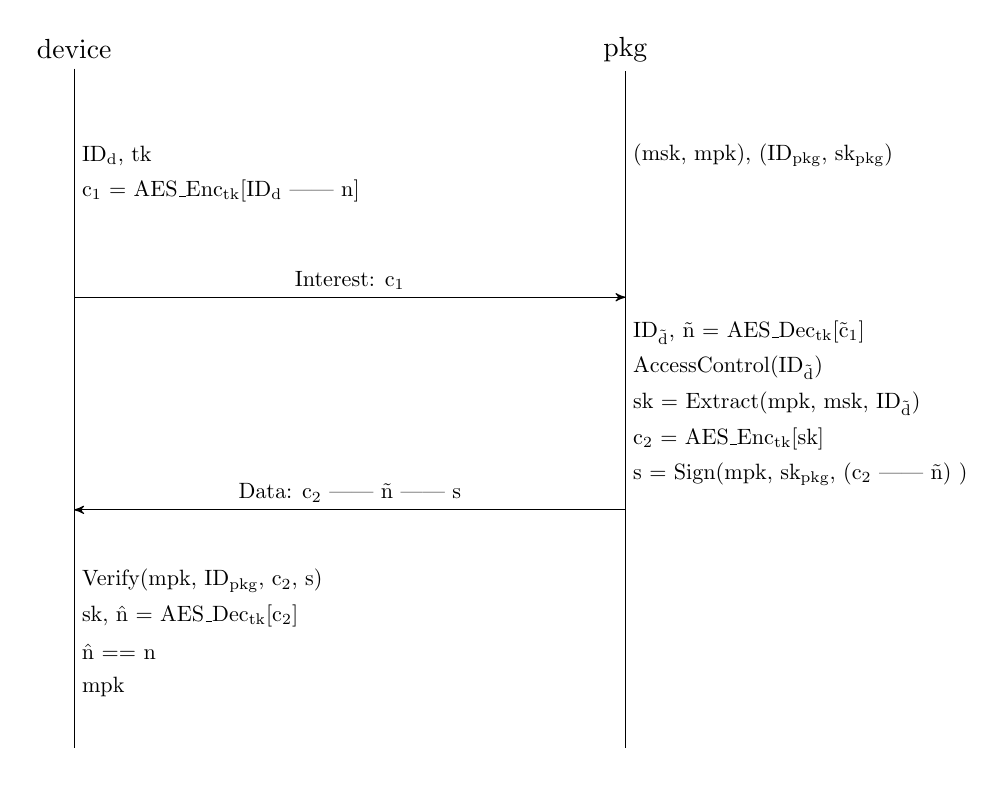
\begin{tikzpicture}[node distance=6cm,auto,>=stealth']
      \node[] (server) {pkg};
      \node[left = of server] (client) {device};
      \node[below of=server, node distance=9cm] (server_ground) {};
      \node[below of=client, node distance=9cm] (client_ground) {};
      %
      \draw (client) -- (client_ground);
      \draw (server) -- (server_ground);

      \draw ($(client)!0.15!(client_ground)$) 
      -- node[above,scale=0.8,right]{ID\textsubscript{d}, tk} 
      ($(client)!0.15!(client_ground)$);
      \draw ($(server)!0.15!(server_ground)$) 
      -- node[above,scale=0.8,right]{(msk, mpk), (ID\textsubscript{pkg}, sk\textsubscript{pkg})} 
      ($(server)!0.15!(server_ground)$);

      \draw ($(client)!0.20!(client_ground)$) 
      -- node[above,scale=0.8,right]{c\textsubscript{1} = AES\_Enc\textsubscript{tk}[ID\textsubscript{d} || n] } 
      ($(client)!0.20!(client_ground)$);
      \draw[->] ($(client)!0.35!(client_ground)$) 
      -- node[above,scale=0.8,midway]{Interest: c\textsubscript{1}} 
      ($(server)!0.35!(server_ground)$);
      \draw ($(server)!0.40!(server_ground)$) 
      -- node[above,scale=0.8,right]{ID\textsubscript{\~{d}}, \~{n} = AES\_Dec\textsubscript{tk}[\~{c}\textsubscript{1}] } 
      ($(server)!0.40!(server_ground)$);
      \draw ($(server)!0.45!(server_ground)$) 
      -- node[above,scale=0.8,right]{AccessControl(ID\textsubscript{\~{d}}) } 
      ($(server)!0.45!(server_ground)$);
      \draw ($(server)!0.50!(server_ground)$) 
      -- node[above,scale=0.8,right]{sk = Extract(mpk, msk, ID\textsubscript{\~{d}}) } 
      ($(server)!0.50!(server_ground)$);
      \draw ($(server)!0.55!(server_ground)$) 
      -- node[above,scale=0.8,right]{c\textsubscript{2} = AES\_Enc\textsubscript{tk}[sk] } 
      ($(server)!0.55!(server_ground)$);
      \draw ($(server)!0.60!(server_ground)$) 
      -- node[above,scale=0.8,right]{s = Sign(mpk, sk\textsubscript{pkg}, (c\textsubscript{2} || \~{n}) ) } 
      ($(server)!0.60!(server_ground)$);
      

      \draw[<-] ($(client)!0.65!(client_ground)$) 
      -- node[above,scale=0.8,midway]{Data: c\textsubscript{2} || \~{n} || s} 
      ($(server)!0.65!(server_ground)$);
      \draw ($(client)!0.75!(client_ground)$) 
      -- node[above,scale=0.8,right]{Verify(mpk, ID\textsubscript{pkg}, c\textsubscript{2}, s) } 
      ($(client)!0.75!(client_ground)$);
      \draw ($(client)!0.80!(client_ground)$) 
      -- node[above,scale=0.8,right]{sk, \^{n} = AES\_Dec\textsubscript{tk}[c\textsubscript{2}] } 
      ($(client)!0.80!(client_ground)$);
      \draw ($(client)!0.85!(client_ground)$) 
      -- node[above,scale=0.8,right]{\^{n} == n } 
      ($(client)!0.85!(client_ground)$);
      \draw ($(client)!0.90!(client_ground)$) 
      -- node[above,scale=0.8,right]{mpk} 
      ($(client)!0.90!(client_ground)$);
  \end{tikzpicture}
  \caption{Device Registration, phase 2. 
  The device sends a Init Interest encrypting nonce \texttt{n} and its \texttt{ID\textsubscript{d}}.
  The device receives the response, decrypts the cipher \texttt{c\textsubscript{1}}, checks if the \texttt{ID\textsubscript{d}} is approved, extracts the secret key corresponding to \texttt{ID\textsubscript{d}}, encrypts the secret key and finally signs the Data.
  }
  \label{fig:init_ibe_2}
\end{figure}


% \begin{figure}[ht]
%   \centering
%   \includegraphics[width=1\textwidth]{Initialization.png}
%   \caption{Initialization IBE}
%   \label{fig:init_ibe_1}
% \end{figure}

Now that the mobile is authenticated, devices can connect to the mobile through e.g. \gls{NFC} for initialization.
This results in a rendezvous authentication between the device and the mobile, and if the mobile is given the authorities to perform initialization (\autoref{access_control}), the new device can join the \gls{PKG}s trust domain.

\subsubsection{Security Analysis}
It is important that the protocol possesses privacy, availability and control properties. 
I shortly present a formal security analysis by modeling the protocol in \gls{spdl} and verifying certain claims through Scyther~\cite{DBLP:conf/cav/Cremers08}.
After that, an informal discussion of the security in the protocol will be presented.

\textit{Scyther}.
The analysis proves that the protocol is confidential, replay and injection resistant, and possesses integrity and authenticity.
All claims made (i.e. \texttt{alive}, \texttt{secret}, \texttt{weakagree}, \texttt{niagree}, \texttt{nisynch}) shows no attacks in Scyther.
The \gls{spdl} code of the protocol can be reviewed in~\autoref{apx:scyther-analysis-dr}.

\textit{Authenticity}.
The protocol holds the required authenticity and integrity. 
The pre-shared temporary random key \texttt{tk} is shared in an assumed secure manner, thus appending an encrypted message to the Init Interest, is used as an authentication for the \gls{PKG}.
Thus the encryption, with the \texttt{tk} as key, protects against \gls{MITM} attacks.
The response \gls{data} is hashed and signed with the \gls{PKG}s \gls{SK} which provides authenticity and integrity for the requesting device.
The signature can easily be verified, and since an adversary do not obtain a polynomial time algorithm that can forge the \gls{SK} the device can be sure that the message is signed by the corresponding ID, which is the ID\textsubscript{PKG} received in the device registration phase 1, seen in~\autoref{fig:init_ibe_1}.
Thus the signature protects against \gls{MITM} attacks.

\textit{Confidentiality}. 
The \gls{SK} will be encrypted with the pre-shared temporary random key \texttt{tk}, and thus the confidentiality is preserved.
An adversary will only be able to know the \gls{MPK}, cipher texts, signatures and both IDs, which is not required to be confidential and not sufficient to compute the \gls{SK} that is extracted. 
The adversary do not obtain a polynomial time algorithm that can compute the \gls{SK} from the known parameters.
Hence an adversary have to obtain a algorithm to compute the secret keys, which is the same polynomial time algorithm as in the sub section above that the adversary do not have access to.

\textit{Replay}.
Since the adversary cannot compute \texttt{tk} nor forge the signature, it cannot send \gls{interest} nor \gls{data} that is captured at any arbitrary point. 
Devices keep track of the nonce corresponding to a data pull, hence a replay with will be detected and thrown away.

\subsection{Deployment Phase}\label{data_pull}
The goal for this protocol is to achieve a secure one-round data pull with authorization and integrity.
For the protocol to work and the data pull to be successful, 1) both devices has to belong to the same trust domain (i.e. has initialized with the same \gls{PKG}) and 2) the requester has to have granted access rights for the resource requested.

As illustrated in~\autoref{fig:health-sensor-system}, the device has joined the \gls{PKG}s trust domain and is ready to communicate with other devices.
This flow is illustrated in~\autoref{fig:data_pull_ibe}.
First the requester has to express an \gls{interest} to the target device asking for a specific resource. 
The \gls{receiver} checks whether the requester has access rights to the requested resource and verifies that the requester is a part of the same trust domain.
If the \gls{receiver} is authorized, the \gls{receiver} responds with the \gls{data} containing the resource. 
The requester signs the \gls{interest} and appends it to the content \gls{name}.
The \gls{receiver} will also do a symmetric encryption on the sensor \gls{data} and do a asymmetric encryption on the \gls{CEK} with the requester's \gls{ID}.
This step is only performed if \gls{data} confidentiality is needed. 
Then the \gls{data} packet is signed and sent.
Finally the requester receives the \gls{data}, verifies the signature and decrypts the sensor \gls{data}.

\begin{figure}[ht]
  \centering
  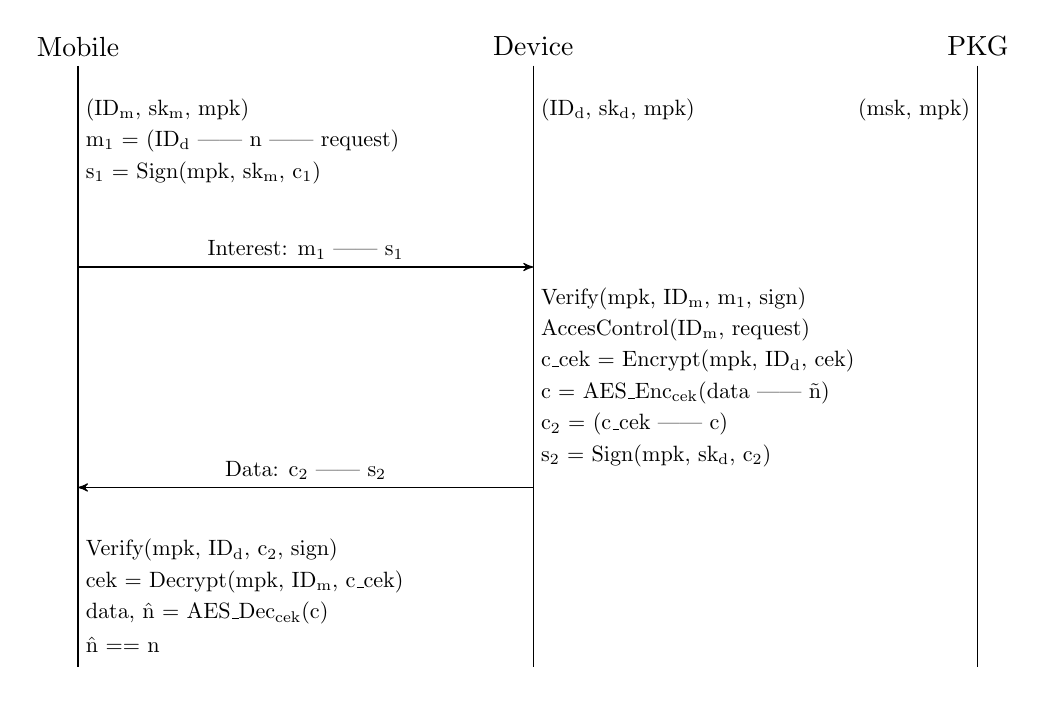
\begin{tikzpicture}[node distance=4.5cm,auto,>=stealth']
      \node[] (server) {PKG};
      \node[left = of server] (client_1) {Device};
      \node[left = of client_1] (client_0) {Mobile};
      \node[below of=server, node distance=8cm] (server_ground) {};
      \node[below of=client_0, node distance=8cm] (client_0_ground) {};
      \node[below of=client_1, node distance=8cm] (client_1_ground) {};
      %
      
      \draw (server) -- (server_ground);
      \draw (client_0) -- (client_0_ground);
      \draw (client_1) -- (client_1_ground);
      
      \draw ($(client_0)!0.10!(client_0_ground)$) 
      -- node[above,scale=0.8,right]{(ID\textsubscript{m}, sk\textsubscript{m}, mpk)} 
      ($(client_0)!0.10!(client_0_ground)$);
      \draw ($(client_1)!0.10!(client_1_ground)$) 
      -- node[above,scale=0.8,right]{(ID\textsubscript{d}, sk\textsubscript{d}, mpk)} 
      ($(client_1)!0.10!(client_1_ground)$);
      \draw ($(server)!0.10!(server_ground)$) 
      -- node[above,scale=0.8,left]{(msk, mpk)} 
      ($(server)!0.10!(server_ground)$);


      \draw ($(client_0)!0.15!(client_0_ground)$) 
      -- node[above,scale=0.8,right]{m\textsubscript{1} = (ID\textsubscript{d} || n || request)} 
      ($(client_0)!0.15!(client_0_ground)$);
      \draw ($(client_0)!0.20!(client_0_ground)$) 
      -- node[above,scale=0.8,right]{s\textsubscript{1} = Sign(mpk, sk\textsubscript{m}, c\textsubscript{1})} 
      ($(client_0)!0.20!(client_0_ground)$);
      \draw[->] ($(client_0)!0.35!(client_0_ground)$) 
      -- node[above,scale=0.8,midway]{Interest: m\textsubscript{1} || s\textsubscript{1}} 
      ($(client_1)!0.35!(client_1_ground)$);
      \draw ($(client_1)!0.40!(client_1_ground)$) 
      -- node[above,scale=0.8,right]{Verify(mpk, ID\textsubscript{m}, m\textsubscript{1}, sign)} 
      ($(client_1)!0.40!(client_1_ground)$);
      \draw ($(client_1)!0.45!(client_1_ground)$) 
      -- node[above,scale=0.8,right]{AccesControl(ID\textsubscript{m}, request)} 
      ($(client_1)!0.45!(client_1_ground)$);
      \draw ($(client_1)!0.50!(client_1_ground)$) 
      -- node[above,scale=0.8,right]{c\_cek = Encrypt(mpk, ID\textsubscript{d}, cek)} 
      ($(client_1)!0.50!(client_1_ground)$);
      \draw ($(client_1)!0.55!(client_1_ground)$) 
      -- node[above,scale=0.8,right]{c = AES\_Enc\textsubscript{cek}(data || \~{n})} 
      ($(client_1)!0.55!(client_1_ground)$);
      \draw ($(client_1)!0.60!(client_1_ground)$) 
      -- node[above,scale=0.8,right]{c\textsubscript{2} = (c\_cek || c)} 
      ($(client_1)!0.60!(client_1_ground)$);
      \draw ($(client_1)!0.65!(client_1_ground)$) 
      -- node[above,scale=0.8,right]{s\textsubscript{2} = Sign(mpk, sk\textsubscript{d}, c\textsubscript{2})} 
      ($(client_1)!0.65!(client_1_ground)$);
      \draw[<-] ($(client_0)!0.70!(client_0_ground)$) 
      -- node[above,scale=0.8,midway]{Data: c\textsubscript{2} || s\textsubscript{2}} 
      ($(client_1)!0.70!(client_1_ground)$);

      \draw ($(client_0)!0.80!(client_0_ground)$) 
      -- node[above,scale=0.8,right]{Verify(mpk, ID\textsubscript{d}, c\textsubscript{2}, sign)} 
      ($(client_0)!0.80!(client_0_ground)$);
      \draw ($(client_0)!0.85!(client_0_ground)$) 
      -- node[above,scale=0.8,right]{cek = Decrypt(mpk, ID\textsubscript{m}, c\_cek)}
      ($(client_0)!0.85!(client_0_ground)$);
      \draw ($(client_0)!0.90!(client_0_ground)$) 
      -- node[above,scale=0.8,right]{data, \^{n} = AES\_Dec\textsubscript{cek}(c)} 
      ($(client_0)!0.90!(client_0_ground)$);
      \draw ($(client_0)!0.95!(client_0_ground)$) 
      -- node[above,scale=0.8,right]{\^{n} == n} 
      ($(client_0)!0.95!(client_0_ground)$);
  \end{tikzpicture}
  \caption{Data pull under deployment. 
  The mobile sends a Sensor Interest to the device appending the request for a resource and a nonce \texttt{n}. 
  The Interest is signed with the mobile's secret key \texttt{sk\textsubscript{m}} and verified by the device. 
  The device checks whether the mobile has a valid capability for the requested resource and encrypts the data if granted.
  The Data response is signed with the device's secret key \texttt{sk\textsubscript{d}}.
  The mobile decrypts of the content encryption key \texttt{cek} and the cipher \texttt{c}, checks whether the received nonce \texttt{\^{n}} is equal to \texttt{n} and finally accepts the data as correct.}
  \label{fig:data_pull_ibe}
\end{figure}

% \begin{figure}[ht]
%   \centering
%   \includegraphics[width=1\textwidth]{DataPull.png}
%   \caption{Mobile performing a data pull from a device in the network.}
%   \label{fig:data_pull_ibe}
% \end{figure}

\subsubsection{Security Analysis}
It is important that the protocol possesses privacy, availability and control properties. 
I shortly present a formal security analysis by modeling the protocol in \gls{spdl} and verifying certain claims through Scyther.
After that, an informal discussion of the security in the protocol will be presented.

\textit{Scyther}.
The analysis proves that the protocol is confidential, replay and injection resistant, and possesses integrity and authenticity.
All claims made (i.e. \texttt{alive}, \texttt{secret}, \texttt{weakagree}, \texttt{niagree}, \texttt{nisynch}) shows no attacks in Scyther. 
The \gls{spdl} code of the protocol can be reviewed in~\autoref{apx:scyther-analysis-dp}.

\textit{Authenticity}.
The protocol holds the required authenticity and integrity. 
The message is hashed and signed with the senders \gls{SK} which provides authenticity and integrity.
The signature can easily be verified by the receiver, and since an adversary do not obtain a polynomial time algorithm that can forge the \gls{SK} one can be sure that the message is signed by the corresponding ID.
Thus the signature protects against \gls{MITM} attacks.

\textit{Confidentiality}. 
All \gls{data} that flows through the \gls{HSS} can be encrypted if necessary. 
When a resource is requested, the \gls{publisher} will do an access control to decide whether the ID\textsubscript{requester} has the right capabilities. 
The \gls{CEK} will be asymmetrically encrypted, and the resource data will be symmetrically encrypted, thus both key and data is confidential and only available to whoever has the corresponding \gls{SK} to the ID\textsubscript{requester}.
An adversary will only be able to know the \gls{MPK}, nonce, request, cipher and both IDs, which is not required to be confidential and not sufficient to compute the resource data. 
The adversary do not obtain a polynomial time algorithm that can compute the resource data from the known parameters.
Hence an adversary have to obtain a algorithm to compute the secret keys, which is the same polynomial time algorithm as in the sub section above that the adversary do not have access to.

\textit{Replay}.
Since the adversary cannot forge the signature, it cannot send \gls{interest} nor \gls{data} that is captured at any arbitrary point. 
This is due to the nonce presence in all packets. 
Devices keep track of the nonce corresponding to a data pull, hence a replay with will be detected and thrown away.

\subsection{Key Distribution using File Synchronization Module}

The Stig wants to have full control over the devices that are a part of the trust domain, and be able to remove a device if necessary.
Each device should have an updated list of all public keys, i.e. every devices' \gls{ID}.
The distribution of this list can easily be achieved by using the \gls{FSM} (\autoref{file-sync} \& \autoref{key-distribution}).
The \gls{PKG} will be the distributor in this synchronization and each device will be a subscriber.


\section{Informal Security Analysis}
In this section an informal security analysis of the whole system is presented.
The assumed threat model will first be presented, along with access control, \gls{CIA}, and trust model.

\subsection{Threat Model}
Threats that I find relevant for the \gls{HSS} can be categorized into three main categories: threats to privacy, threats to availability and threats to control.
I assume the following threat model:
\begin{enumerate}
  \item An adversary might try to eavesdrop information (privacy).
  \item An adversary might try to send bogus commands, e.g. injection, replay and \gls{MITM} (control).
  \item Jamming, node compromise (such as theft of mobile) and \gls{DoS} (availability).
\end{enumerate}

I assume that the \gls{PKG} cannot be compromised by any adversary, and thus the \gls{MSK} will always be hidden from any adversaries. 
However, it is extremely important that the machine which plays the role of the \gls{PKG} is secured in a physical matter, as well as remote secureness. 
The \gls{PKG} is the single point of failure in the whole system.

An idea introduced by Aaditeshwar Seth and Srinivasan Keshav in~\cite[Section 5.4]{Seth:2005:PSD:1897159.1897165} is to avoid storing the \gls{SK}s in devices that is more likely to be lost or stolen, e.g. a mobile.
Using \gls{HIBC}, one can extend the key hierarchy by another level that is time-based.
These time-based keys can then be downloaded to the mobile on a daily basis, hence the time the mobile will be compromised is reduced.

\subsection{Access Control}\label{access_control}
Since the ID\textsubscript{device} is appended to the \gls{interest} and the \gls{interest} is signed by the corresponding SK\textsubscript{device}, the \gls{ID} of the device can easily be authenticated. 
When a device retrieves an \gls{interest} for its sensor \gls{data}, there should be an authorization mechanism. 
One can argue that once a device has been authenticated in the \gls{PKG}s trust domain, everyone in the domain can be sure that the device will not abuse the information or functionalities available. 
However, due to scalability this is not a secure way to handle access control. 
If a device does not need a privilege, it does not need it.
Hence it should not have it. 
That is the least privilege access principle, which is default in Capability Based Approach to \gls{IoT} Access Control~\cite{DBLP:conf/imis/GusmeroliPR12}.
This approach has some additional benefits for the \gls{HSS}, such as

\begin{itemize}
  \item delegation support - 
  A device can grant access rights to other devices, as well as granting the right to further delegate these rights to a third device.
  \item capability revocation - 
  If the \gls{PKG} have granted delegation rights to a mobile, and the mobile is not found trustworthy after a while, the capabilities issued by the mobile can easily be revoked.
  \item information granularity - 
  Specific resources from a device can be granted access to in different granularity.
\end{itemize}

Another solution can be an \gls{ACL} based approach equivalent to what Wentao Shang et al. did in~\cite{DBLP:journals/network/ShangDMBZ14}.

\subsection{Confidentiality}
The confidentiality is achieved by doing asymmetric encryption on a \gls{CEK} that is used for symmetric encryption on the content.
As explained in the sequence diagram (\autoref{fig:data_pull_ibe}) presented in the above sections, each \gls{interest} appends the requester's ID (\autoref{eq:mapping-id-name-pk}).
Since the ID\textsubscript{requester} always is appended it can always be used to do asymmetric encryption, hence all \gls{CEK}s can be encrypted only for the requesting device, and thus the confidentiality in the system can always be achieved.

\subsection{Integrity and Authenticity}
Each device will obtain a secret key allocated by its superior \gls{PKG}, as explained in~\autoref{ibc}.
With the concept from~\autoref{rendezvous_authentication} together with the \gls{PKG}s \gls{MPK}, you can trust that the device is authorized for the \gls{PKG}s trust domain. 
Hence all signed packets can be verified by anyone with the \gls{MPK}.
In this setting, a verified signature acts as an assurance of authentication and integrity. 

Every \gls{interest} has a timestamp attached to the \gls{name} (e.g. \path{/ndn/no/ntnu/device/name2/sensorPull/1429710873778}), i.e. milliseconds from \texttt{UTC} \texttt{1970-01-01} \texttt{00:00:00}, that can be used for protection against replay attack. 

\subsection{Availability}
This is a harder problem to solve.
The network is purely wireless, hence vulnerable to jamming. 
An adversary could try to send infinite \gls{interest}s to a device with an invalid signature, hence the device may be overloaded with work and might run out of battery fast.
Therefore one should check the \gls{MPK} before doing any crypto.
This is also why I have chosen to append the MPK in the packet~\autoref{fig:sensor_interest-data}. 

\subsection{Trust Model}
For a system to be secure, cryptography together with trust is essential. 
The \gls{HSS} trust model is built upon trusting a centralized authority, typically the user's home server, rendezvous authentication and \gls{IBC}.
The fact that it runs over \gls{NDN} makes it easier to achieve security goals and usability for third party developers.

The \gls{PK} is the \gls{name} of the device, and all content published by the device will begin with this \gls{name}, hence it is easy to verify that the \gls{publisher} is the owner of the content.
To be able to verify and encrypt messages, the device need the MPK\textsubscript{PKG} and the ID of the user it wants to communicate with. 
If allowed by the PKG, the public parameters MPK\textsubscript{PKG} is public for everybody that is not a part of the trust domain. 
To be able to sign and decrypt messages the device have to be a member of the trust domain and be issued a secret key mapping to the ID\textsubscript{device}.
Each device builds its trust on other devices based on that it has been verified by an administrator that controls the \gls{PKG}.

\chapter{Implementation and Testing}

\section{FileSync.py application}
Application goal explained in~\autoref{file-sync}
Appendix code~\autoref{apx:file-sync-code}

FileSync is a python application that will synchronize all files in a specified path, with all participants within the synchronization room.

\section{Application.py}
Application flow explained in~\autoref{sensor-application}

\subsection{Packet Design}
Initialization packets are limited to the structure in~\autoref{fig:init_interest-data}
Sensor packets are limited to the structure in~\autoref{fig:sensor_interest-data}
\begin{description}
	\item[Init Interest]
	\item[Init Data]
	\item[Sensor Interest]
	KeyLocator can be of type Name. 
	As described in the \gls{NDN} Packet Format, generally this field can be used to specify where to download the certificate used to sign the Interest.
	However, in our trust model we use this field to publish the requesters Name, i.e. the requesters public key. 
	\item[Sensor Data]
\end{description}

\begin{figure}[ht]
  \centering
  \includegraphics[width=1\textwidth]{init_interest-data.png}
  \caption{Initialization Interest and Data}
  \label{fig:init_interest-data}
\end{figure}

\begin{figure}[ht]
  \centering
  \includegraphics[width=1\textwidth]{sensor_interest-data.png}
  \caption{Sensor Interest and Data}
  \label{fig:sensor_interest-data}
\end{figure}
\chapter{Discussion}
In this chapter it will be discussed 

\section{Identity-Based Encryption}
One suggestion has been to add a monthly timestamp~\cite{DBLP:journals/iacr/BoldyrevaGK12} ~\cite{DBLP:conf/ctrsa/LibertV09} \todo{find better cite} to the name, but the the \gls{PKG} has to renew private keys for everybody each month. 
This solution scales very badly.
With the \gls{PKG}s Name Sync application, every user will be notified when a identity is revoked.
There is no use for periodically checking names.

\section{Trusting Trusted Third Party in Identity-Based Cryptography}
Issues of trusting the \gls{PKG}, i.e. a \gls{TTP}. 
If the \gls{PKG} is compromised by an adversary, the adversary will retrieve all private keys corresponding to all IDs that used the compromised \gls{PKG}. 
Do every ID trust the \gls{PKG}? Suspicion of \gls{MITM}, where the \gls{PKG} is the adversary, will always be a problem for a user.
Secure channel for private key exchange. 
\chapter{Conclusion and Future Work}\label{chp7:conclusion}

\section{Future Work}



%\chapter{NDN node 23 - NTNU}

\section{NDN node 23 - NTNU}
Node 23 in NDN testbed

\begin{figure}[ht]
  \centering
  \includegraphics[width=1\textwidth]{ndn-map.png}
  \caption{NDN Map}
  \label{fig:ndn-map}
\end{figure}

%% include here the other chapters

%% References
%\include{references}
\renewcommand*{\bibname}{References}
%\bibliographystyle{ieeetr}
\bibliographystyle{alpha}
\bibliography{main}

% Uncomment the following if you have any appendix
\appendix
\addtocontents{toc}{%
 \protect\vspace{1em}%
 \protect\noindent \bfseries \appendixtocname\protect\par
 \protect\vspace{-.5em}%
}
\renewcommand{\chaptername}{\appendixname}
% include below possible appendices (chapters)
%\include{appendix}
\chapter{ChronoSync}\label{apx:chronosync}

Since \gls{NDN} provides multicast in the network layer as explained in~\autoref{fig:ndn-multicast}, we do not have to think of network load in the same way as in \gls{IP}.  
To achieve distributed synchronization of a \gls{data}set, the \gls{NDN}-team has developed ChronoSync, a decentralized synchronization framework over \gls{NDN}. 
ChronoSync assumes that a group of nodes knows the \gls{name} of a \gls{synchronization_group}, e.g \path{/ndn/broadcast/FileSync-0.1/<group_room>/}.
The synchronication application is built upon state digests, which is that each participating node stores a hash of its current \gls{data}set. 
Each node in a ChronoSync application broadcasts its sync state in a Sync \gls{interest} (e.g. \path{/ndn/broadcast/FileSync-0.1/<group_room>/<state>}).
When a node receives a Sync \gls{interest}, it will inspect the state of the \gls{interest}, and compare with its own state.
Each node holds a state tree that is used to detect new and outdated states.
If the incoming \gls{interest} state is equal to the receiving node's state, the node has no reason to do anything, as the system is in a \textit{stable state} from the node's point of view.
If not, the receiving node has to find out whether the incoming \gls{interest} is 1) a state the node itself has been in, or if its 2) a new state.
In case of 1), the receiving node has new \gls{data} and should provide the new content as a response to the incoming \gls{interest}. In case of 2), the receiving node should send out a Recovery \gls{interest} for the new state.

\begin{enumerate}
  \item \textit{Sync \gls{interest}} is an \gls{interest} that a participating node sends out to discover new \gls{data}.
  \item \textit{Sync \gls{data}} is a response to 1), if a participating node has new \gls{data}.
  \item \textit{Recovery \gls{interest}} is an \gls{interest} sent out if a node discovers that another node has a newer state.
  \item \textit{Recovery \gls{data}} is a response to 3).
\end{enumerate}

When the group is in a stable state, each Sync \gls{interest} is equivalent, hence only one entry at each router's \gls{PIT} is created, forming a temporary multicast three.
This \gls{interest} is periodically sent out from each subscriber maintaining the multicast three, resulting in that the producer has the possibility to answer the Sync \gls{interest} with Sync \gls{data} whenever the producer has a new \gls{data}set.

ChronoSync is only taking care of \gls{data} discovery, and leaves other logic to the application that is using ChronoSync. 
Such logic can be e.g. what should happen when a new participant enters the room.
Should all history be downloaded? 
Or who is allowed to publish content in each \gls{synchronization_group}?

ChronoSync is explained in detail here~\cite{DBLP:conf/icnp/ZhuA13}.
\chapter{Code}\label{apx:code}

\section{Public Key Sync application}

Using watchdog to observe files

\begin{lstinputlisting}
[language=Python]{code/pk-sync.py}
\end{lstinputlisting}

\end{document} 
